\documentclass[10pt]{article}
\usepackage[a4paper,margin=22mm]{geometry}
\usepackage[T1]{fontenc}
\usepackage[utf8]{inputenc}
\usepackage{lmodern,amsmath,amssymb,graphicx,float,fancyhdr,xcolor}
\usepackage{fancyvrb,etoolbox}
\BeforeBeginEnvironment{verbatim}{\par\noindent\begin{minipage}{\linewidth}}
\AfterEndEnvironment{verbatim}{\end{minipage}\par}
\usepackage[unicode,hidelinks]{hyperref}
\DeclareUnicodeCharacter{2192}{\ensuremath{\rightarrow}}
\providecommand{\textt}[1]{\texttt{#1}}
\providecommand{\tightlist}{\setlength{\itemsep}{0pt}\setlength{\parskip}{0pt}}
\setlength{\parindent}{0pt}
\setlength{\parskip}{0.6em}
\setlength{\headheight}{41pt}
\setlength{\emergencystretch}{3em}
\pagestyle{fancy}
\lhead{
\includegraphics[width=2.5cm]{edem_logo.jpg}}
\rhead{Computer Science -- Rehearsal}
\cfoot{\thepage}
\let\OldSection\section
\renewcommand{\section}{\clearpage\OldSection}
\begin{document}
\begin{center}
{\LARGE\bfseries Computer Science\\Partial exam rehearsal -- Student version\par}
\vspace{1em}
IGE -- 1st Year\\Class practice
\end{center}
\textbf{Suggested duration:} 1 hour 45 minutes, followed by class discussion.

Answer each question and show your reasoning. For multiple-choice questions, choose one answer and justify it. Write your answers on separate sheets. Questions are in English.

\textbf{Content.} This rehearsal covers three units. Unit 1 focuses on binary representation, CPU instructions and register states (2 points, 20\%). Unit 2 covers Python imports, numeric operations, Boolean conditions, \texttt{if-elif-else}, loops and lists (3 points, 30\%). Unit 3 covers Arduino programming, error detection, digital inputs and outputs, and an LCD scoreboard (5 points, 50\%). These weights are indicative for this academic year and should be used as a guide when preparing for the exam.

\section*{Unit 1 Problems (2.0 points total)}

\subsection*{Q1 - CPU execution}
A processor has four registries, labeled R0, R1, R2, and R3 and the following set of operation codes: 
\begin{enumerate}
    \item \texttt{0001} Addition
    \item \texttt{0010} Substraction
    \item \texttt{1100} Multiplication
    \item \texttt{1101} Integer Division
    \item \texttt{1110} Modulo (reminder after Integer division)
\end{enumerate}
The 10-bit instruction is formatted as follows. 

\texttt{Opcode(4) | Dest(2) | Src1(2) | Src2(2)}

For example, the instruction \texttt{1110 00 01 10} means "calculate the reminder after Integer division of the value of registry R1 divided by the value of registry R2 (R1 modulo R2), and store the value in registry R0".

The initial value in the registers are in table \ref{tab:initial_state}: 

\begin{table}[H]
    \begin{tabular}{ll}
        R0 & \textt{0b1011}\\
        R1 & \textt{0b1000}\\
        R2 & \textt{0b0010}\\
        R3 & \textt{0b0000} \\ 
    \end{tabular}
    \caption{Initial states}
    \label{tab:initial_state}
\end{table}



Answer the following questions: 
\begin{enumerate}
    \item Convert to decimal the values in registry (prefixed with \verb|0b|). \textbf{(0.5 pts)}
    
\vspace{1.2cm}
    \item Write the instruction to add the values in registries R1 and R2 and store it back in registry R2. This instruction will be instruction 1. \textbf{(0.2 pts)}\\
    
\vspace{1.2cm}
    \item Consider the following instructions:
    \begin{itemize}
        \item Instruction 2: 0010000001
        \item Instruction 3: 1110110100
    \end{itemize}
    Explain what every instruction will do.(0.3 pts)

\vspace{1.2cm}
    \item Using the initial state, apply instruction1, instruction2 and instruction3. Show the state
of the registers after the execution of every instruction. \textbf{(1 pts)}      

\vspace{1.2cm}
\end{enumerate}


\section*{Unit 2 -- Python (3 points total)}
\subsection*{Python Q1 -- Scenario 4 -- Requesting a concise import (0.375 pt)}
A financial analyst only needs \texttt{sqrt()} from the \texttt{math}
module and wants to call it without the \texttt{math.} prefix. Which
option meets the requirement?

A. \texttt{import\ math} followed by \texttt{math.sqrt(81)}\\
B. \texttt{import\ math\ as\ sqrt} followed by \texttt{sqrt(81)}\\
C. \texttt{from\ math\ import\ sqrt} followed by \texttt{sqrt(81)}\\
D. \texttt{from\ sqrt\ import\ math} followed by \texttt{sqrt(81)}

\textbf{Your choice:}\\
\textbf{Which name becomes available?}


\subsection*{Python Q2 -- Scenario 2 -- Packing devices (0.375 pt)}
A warehouse must pack 137 devices into boxes that hold 12 devices each.
The manager needs the number of complete boxes and unpacked devices.
Which solution is most appropriate?

\begin{enumerate}
\def\labelenumi{\Alph{enumi}.}
\tightlist
\item
\end{enumerate}

\begin{verbatim}
boxes = 137 / 12
remaining = 137 / 12
\end{verbatim}

\begin{enumerate}
\def\labelenumi{\Alph{enumi}.}
\setcounter{enumi}{1}
\tightlist
\item
\end{enumerate}

\begin{verbatim}
boxes = 137 // 12
remaining = 137 % 12
\end{verbatim}

\begin{enumerate}
\def\labelenumi{\Alph{enumi}.}
\setcounter{enumi}{2}
\tightlist
\item
\end{enumerate}

\begin{verbatim}
boxes = 137 % 12
remaining = 137 // 12
\end{verbatim}

\begin{enumerate}
\def\labelenumi{\Alph{enumi}.}
\setcounter{enumi}{3}
\tightlist
\item
\end{enumerate}

\begin{verbatim}
boxes = int(137 / 12)
remaining = 137 - 12
\end{verbatim}

\textbf{Your choice and justification:}


\clearpage
\subsection*{Python Q3 -- Scenario 4 -- Secure document access (0.375 pt)}
A user may open a confidential document when they have permission and
their account is not suspended. The following code illustrates how the
condition will be used. Replace \texttt{<condition>} with one of the
options below. Which condition states the requirement most directly?

\begin{verbatim}
has_permission = True
account_suspended = False

if <condition>:
    print("Access granted")
else:
    print("Access denied")
\end{verbatim}

A. \texttt{has\_permission\ or\ not\ account\_suspended}\\
B. \texttt{has\_permission\ and\ not\ account\_suspended}\\
C. \texttt{not\ has\_permission\ and\ account\_suspended}\\
D. \texttt{has\_permission\ and\ account\_suspended}

\textbf{Your choice and a test that should deny access:}


\subsection*{Python Q4 -- B7. Diagnosing an index error (0.375 pt)}
An AI assistant generates the following loop and Python raises
\texttt{IndexError} on the last iteration:

\begin{verbatim}
for index in range(len(values) + 1):
    print(values[index])
\end{verbatim}

Which explanation is most accurate?

A. Lists cannot be used inside \texttt{for} loops.

B. \texttt{range()} includes its stop value.

C. The \texttt{+\ 1} creates an index equal to the list length, which is
outside the valid range.

D. The loop must begin at index \texttt{1}.


\clearpage
\subsection*{Python Q5 -- A7. Prioritise outcomes (0.75 pt)}
A support request should receive exactly one classification:
\begin{enumerate}
\item \texttt{"Critical"} when the service is unavailable.
\item \texttt{"High"} when data may be lost.
\item \texttt{"Medium"} when response time exceeds 5 seconds.
\item \texttt{"Normal"} otherwise.
\end{enumerate}
Implement the policy with \texttt{if-elif-else}. Create a case where several
conditions are true and explain why only one branch runs.

\begin{verbatim}
service_unavailable = False
possible_data_loss = True
response_time = 8.2

# Implement and print the classification here.
\end{verbatim}


\clearpage
\subsection*{Python Q6 -- A5. Preserve a running series (0.75 pt)}
A new online service begins with \texttt{200} registered users (stored in
\texttt{initial\_users}). A list contains the new users gained each week
(\texttt{new\_users\_by\_week} stores the new users for each week).

Create \texttt{total\_users\_by\_week} so that it contains the initial
total followed by the total after every week.

\begin{verbatim}
initial_users = 200
new_users_by_week = [25, 30, 20, 35]
total_users = initial_users
total_users_by_week = [initial_users]

# Update total_users for every week.
# Preserve every updated total in total_users_by_week.

print(total_users_by_week)
\end{verbatim}


\section*{Unit 3 Problems (5 points total)}

\subsection*{Q1 — Error Detection \& Correction (1.5)}
Consider the following code, it contains several syntax/logic errors.
\begin{verbatim}
const int led1 = 11
const int led2 = 2;
const int btn = 11;

void setup() {
    pinMode(led1, OUTPUT)
    pinMode(led2, OUTPUT);
    pinMode(btn, OUTPUT);
}

void setup() {
if (digitalRead(btn) = HIGH) {
    pattern = !pattern;
    }
    if (pattern = true) {
        digitalWrite(led1, HIGH);
        digitalWrite(led2, LOW);
    } else {
        digitalWrite(led1, HIGH);
        digitalWrite(led2, HIGH)
        delay(300);
        digitalWrite(led1, LOW);
        digitalWrite(led2, LOW);
    }
    delay(300)
}
\end{verbatim}

Solve the following items:
\begin{enumerate}
    \item Find all 9 errors in the code (0.5 pts).

\vspace{1.2cm}
    \item For every error, explain why it’s an error and how to fix it (0.5 pts).

\vspace{1.2cm}
    \item Explain what the corrected code is doing (0.5 pts).

\vspace{1.2cm}
\end{enumerate}

\clearpage\subsection*{Q2 - Referee table (1.5)}
The following schematic represents your prototype board. The integrated protoboard includes 2 push buttons, labeled as B1, and B2, and two (pull-down resistors). The objective of the prototype is to provide an electronic table to keep track of the score in a football match. Push-button B1 is used to control the score of the local team  and B2 is used to control the score of the visiting team (1 push increases the score in 1). 
\begin{figure} [H]
    \centering
    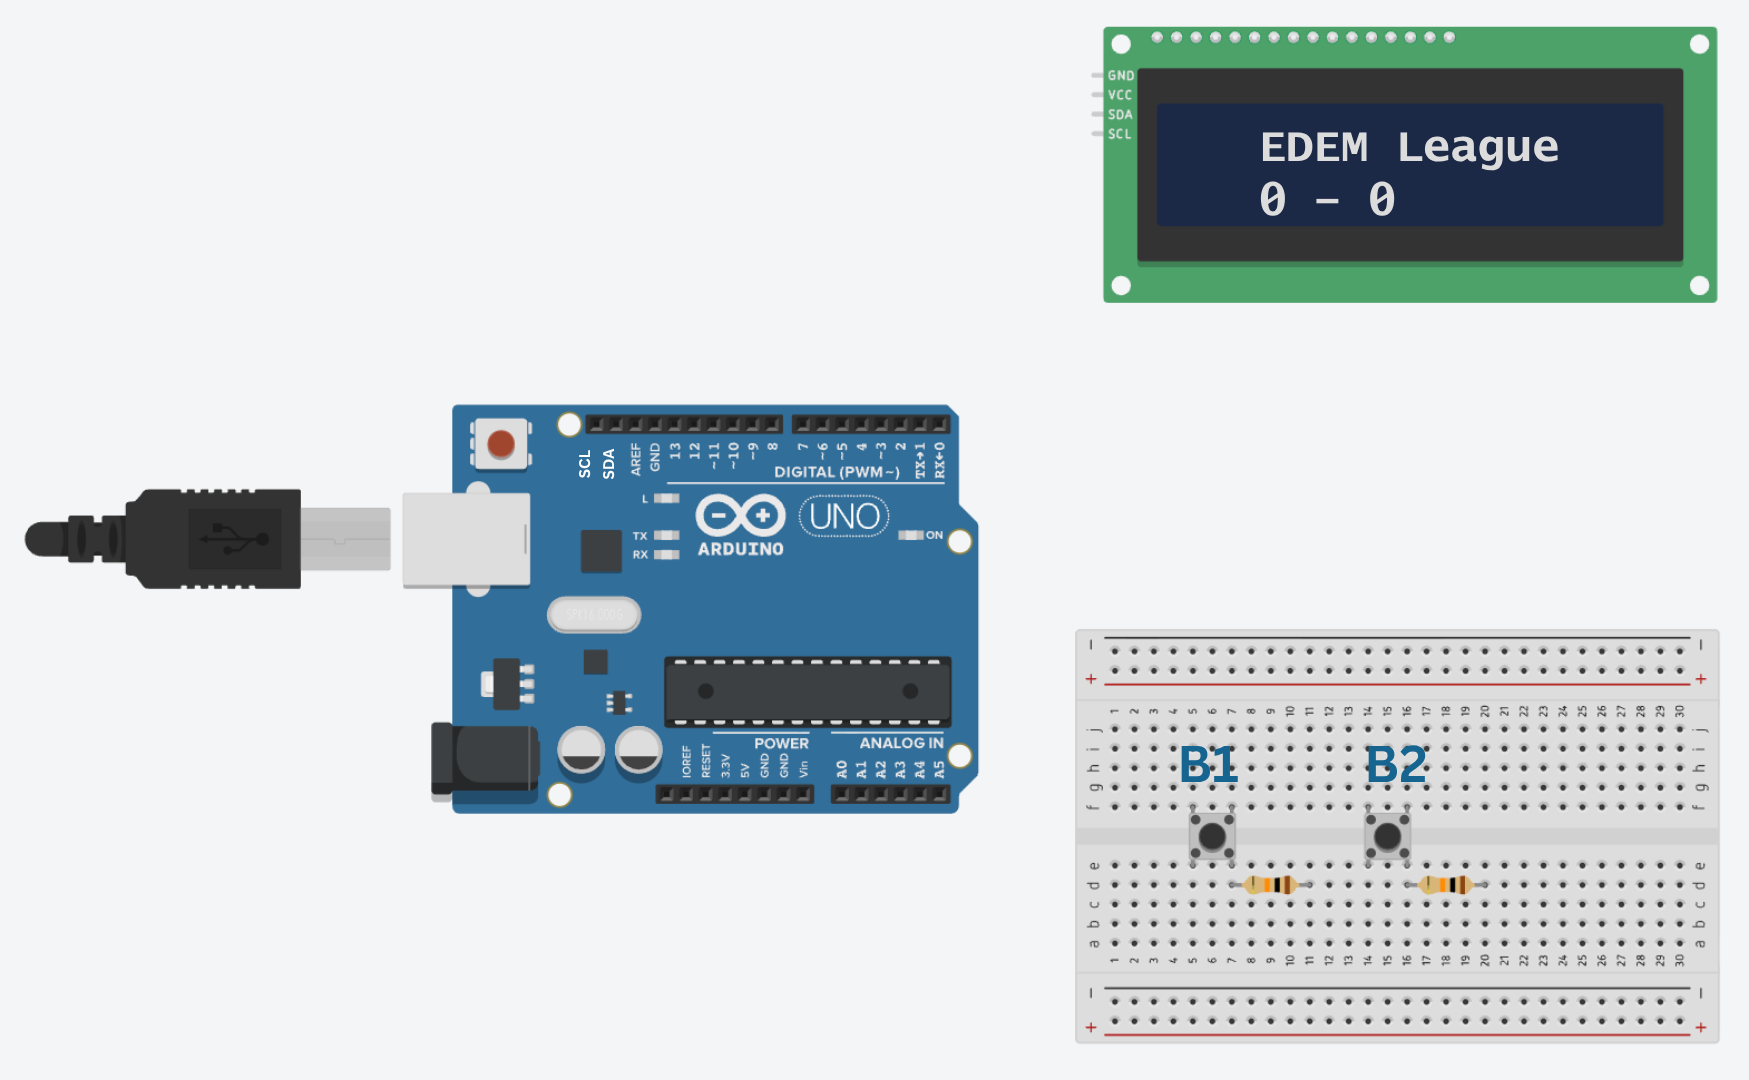
\includegraphics[width=1\linewidth]{Circuit_student.png}
    \caption{EDEM League electronic table}
    \label{fig:placeholder}
\end{figure}

Based on the provided information and diagram, follow the instructions below to complete the
wiring of the prototype.
\begin{enumerate}
    \item Draw over the diagram the wires needed to connect the circuit (0.5 pts)
    \begin{enumerate}
        \item Complete the variables, constants needed. (0.5 pts)

\vspace{1.2cm}
        \item Complete the setup function (1 pts)
\vspace{1.2cm}
        \item Complete the loop function (1.5 pts)

\vspace{1.2cm}
    \end{enumerate}
\end{enumerate}

To write the code, you can base it on this example of how an LCD screen works, provided as an
example in the next page.

\clearpage\subsection*{Example code}
This code will turn on the LCD screen, write ”hello world” in the first line, and then, in the
second line, it writes, every second, the amount of seconds that it has been working. You can
use this code as inspiration to write the code of the last exercise.

\begin{verbatim}
#include <Adafruit_LiquidCrystal.h>
int seconds = 0;
Adafruit_LiquidCrystal lcd_1(0);
void setup()
{
    lcd_1.begin(16, 2);
    lcd_1.print("hello world");
}
void loop()
{
    lcd_1.setCursor(0, 1);
    lcd_1.print(seconds);
    delay(1000); // Wait for 1000 milliseconds
    seconds += 1;
}    
\end{verbatim}

\end{document}
